\documentclass{article}
\usepackage{fancyhdr}
\usepackage{amsmath}
\usepackage{enumerate}
\usepackage{graphicx}
\usepackage{caption}
\usepackage{subcaption}
\pagestyle{fancy}
\lhead{Trevor Slaton (tms45)\\Joseph Vokt (jpv52)}
\rhead{Machine Learning (CS 4780)\\Homework \#2: Due Sept. 24, 2013}

\begin{document}
\thispagestyle{fancy}

\section{Model Selection and Validation}

\begin{enumerate}[(a)]
\item $S_{train}$ accuracy: 22/24. $S_{test1}$ accuracy: 8/10. $S_{test2}$ accuracy: 16/20. 
\item $S_{train}$ accuracy: 24/24. $S_{test1}$ accuracy: 8/10. $S_{test2}$ accuracy: 15/20. 
\item Let $x=\frac{(n_{01}-n_{10})^2}{n_{01}+n_{10}}$ where $n_{01}$ corresponds to the number of cases which were missclassified by the decision tree hypothesis and not the linear hypothesis, and $n_{10}$ corresponds to the number of cases which were missclassified by the linear hypothesis but not the decision tree hypothesis. For $S_{test1}$, $n_{01}=1$ and $n_{10}=1$, so $x=0$. Using matlab chi2cdf(x,1), we get a p-value of 0. Thus we can't say that one model generalizes any better than the other.
\item For $S_{test2}$, $n_{01}=3$ and $n_{10}=2$, so $x=\frac{1}{5}=.2$. Using matlab chi2cdf(x,1), we get a p-value of 0.3453. Thus we can't confidently say that one model generalizes any better than the other.
\item The accuracy for $S_{test1}$ is the same for both the linear hypothesis and decision tree. The $\chi^2$ statistic for the McNemar test for $S_{test1}$ comparing the two hypotheses confirms that there is no significant difference in how well they generalize. The accuracy for $S_{test2}$ is slightly higher for the linear hypothesis than the decision tree. However, the $\chi^2$ statistic for the McNemar test for $S_{test2}$ comparing the two hypotheses reveals that we are not justified in claiming that one hypothesis generalizes better than the other. 

Although the results for the two McNemar tests were different, the conclusion is the same. Unlike for $S_{test1}$, the decision tree hypothesis does separately misclassify more examples in $S_{test2}$ than does the linear hypothesis, but the difference between their misclassification rates is still shown by the McNemar test to be insignificant. In order to determine that results are significant at a confidence level of 95\%, the $\chi^2$ statistic for the McNemar test must exceed the critical value 3.84, which mathematically requires both a sizable discrepancy between the separate misclassifications $n_{01}$ and $n_{10}$ and a large total number of misclassifcations (e.g. $n_{01}=40,n_{10}=60$). In both cases for this question, we have neither.

\end{enumerate}

\section{Model Averaging with Decision Trees}

\begin{enumerate}[(a)]
\item Individal decision tree:

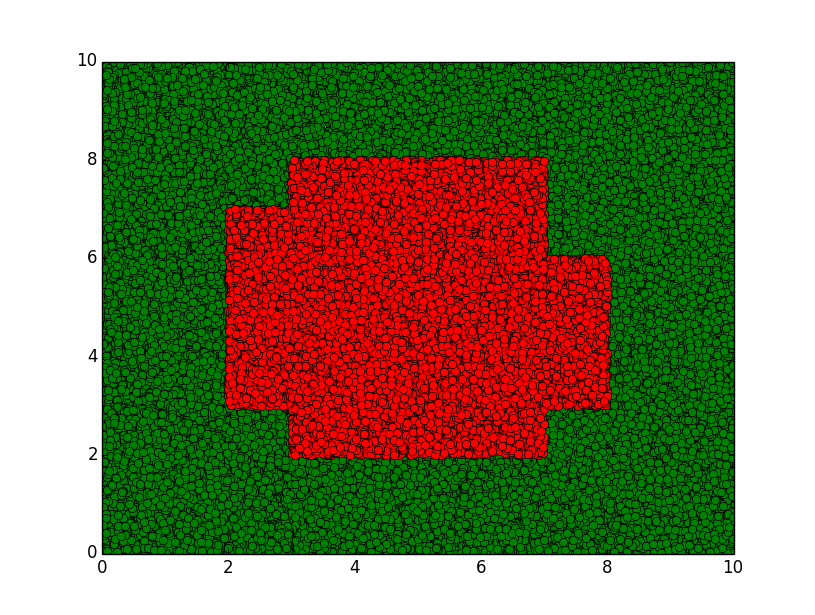
\includegraphics[scale=.5]{2a.png}

\item Two trees that are particularly illustrative examples of overfitting.

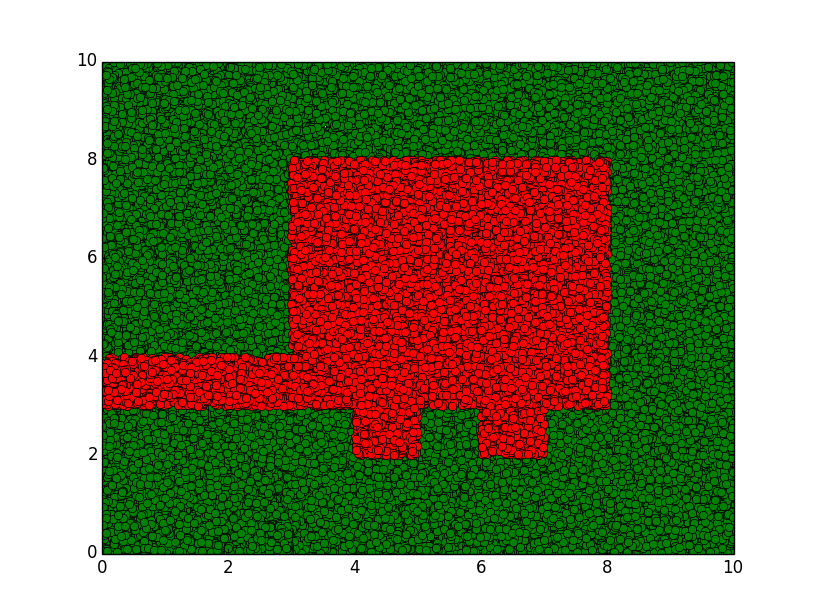
\includegraphics[scale=.5]{2b-herp1.png}

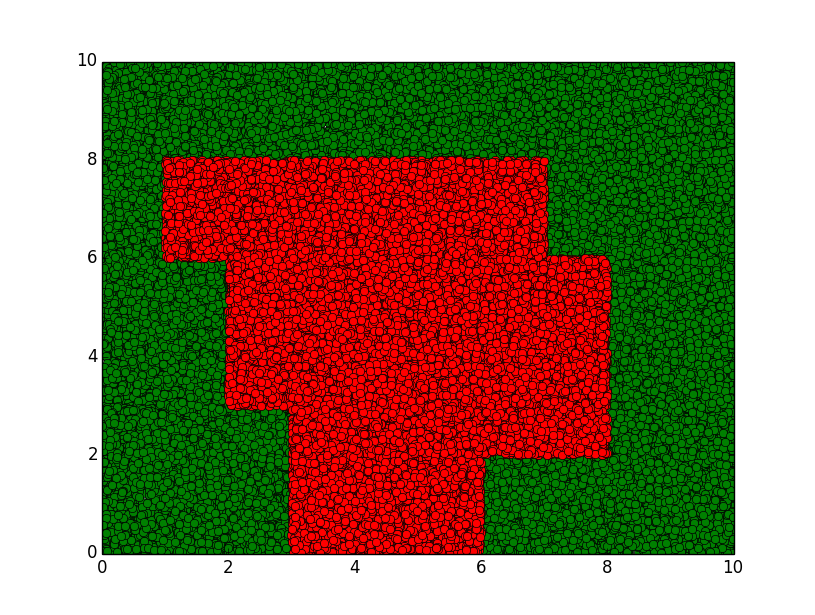
\includegraphics[scale=.5]{2b-herp2.png}

Averaging decision trees:

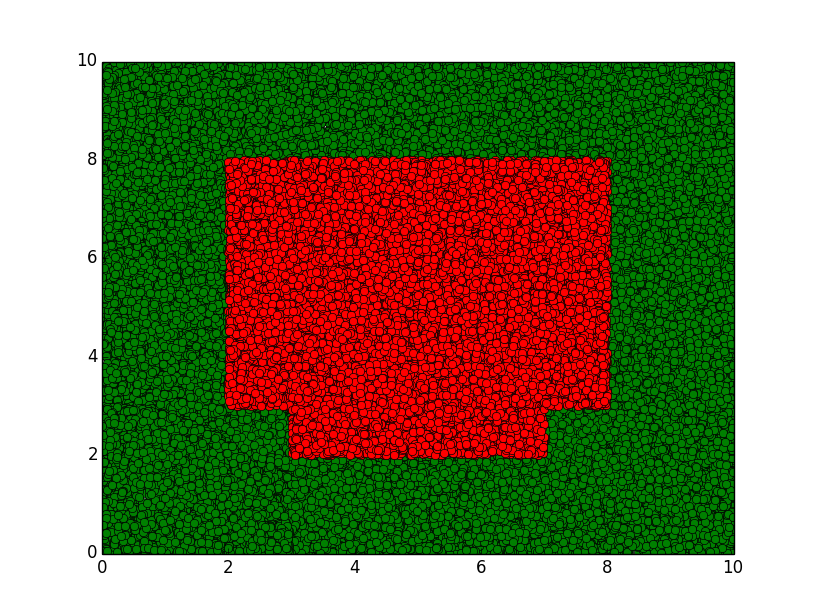
\includegraphics[scale=.5]{2b.png}

Both the combined and the individual are close to the true boundary (within reason, as we can only split on integers). However, many of the 101 the individual trees appear to have suffered from training on less data, meaning that they have overfit a subset of the full training data that is not representative of the true boundary. By training many trees, we average out the error and the outliers cancel out. If we had a better granularity for potential splitting thresholds, our decision trees would have been much better at approximating the true boundary.

\item Show that a prediction can be expressed as follows:
\[\hat{y} = sign\left(\sum_i^n y_i K ( x_{test} , x_i )\right)\]
A test instance, $x_{test}$ can end up in one and only one leaf. Let $k$ be the number of training instances in that leaf. This means that the similarity measure $K(x_{test},x_i)$ will be nonzero for exactly $k$ training instances $x_i$. If for example all training instances in that leaf are labeled as $+$, we get
\[\hat{y} = sign\left(\sum_i^k 1/k \right)=sign(1)=+\]
If for example all training instances in that leaf are labeled as $-$, we get
\[\hat{y} = sign\left(\sum_i^k -1/k \right)=sign(-1)=-\]
If the majority of training instances in that leaf are $+$, then the test instance is labeled as $+$. If the majority of training instances in that leaf are $-$, then the test instance is labeled as $-$. If there are an equal number, we will have to flip a coin.
\item Show that averaging predictions from $M$ different trees,
\[\hat{y} = sign\left(\frac{1}{M}\sum_j^M\sum_i^n y_i K_j ( x_{test} , x_i )\right)\]
can be expressed as follows:
\[\hat{y} = sign\left(\sum_i^n y_i \tilde{K} ( x_{test} , x_i )\right)\]
Proof:
\begin{align*}
\hat{y} &= sign\left(\frac{1}{M}\sum_j^M\sum_i^n y_i K_j ( x_{test} , x_i )\right)\\
&=  sign\left(\sum_i^n y_i \frac{1}{M}\sum_j^M K_j ( x_{test} , x_i )\right)\\
&= sign\left(\sum_i^n y_i \tilde{K} ( x_{test} , x_i )\right)
\end{align*}
where
\[\tilde{K}( x_{test} , x_i )=\frac{1}{M}\sum_j^M K_j ( x_{test} , x_i )\]
Intuitively, to label test instance $x_{test}$ we are measuring which is greater: \\
(1) $\sum_i \tilde{K}( x_{test} , x_i )$ where $i$ is such that $x_i$ is labeled with a plus, or \\
(2) $\sum_i \tilde{K}( x_{test} , x_i )$ where $i$ is such that $x_i$ is labeled with a minus. \\$\tilde{K}( x_{test} , x_i )$ represents the average $K$ among all $M$ different trees. If $x_i$ has a $+1$ label, it would contribute to the first term, and if it has a $-1$ label it would contribute to the second. In other words, we label $x_{test}$ based on whether we have more decision trees that predict $+1$ or $-1$.
\end{enumerate}
\section{Text Categorization with Decision Trees}

\begin{enumerate}[(a)]
\item \emph{Decision Tree I.} Test error on the test set groups.test: 28.85\% (71.15\% accuracy)
\item \emph{Informative words.} Words from groups.vocab corresponding to the splits at the top 2 levels of the tree were "windows" (id 1289) at level 1 and "car" (id 603) and "christian" (id 1090) at level 2. These results make sense given that they should be fairly revealing of the subject matter in one of the following categories: auto ("car"), computers ("windows"), religion ("christian"), and sports. Words corresponding to the splits at the bottom 2 levels of the tree were "an" (id 1847), "attitude" (id 1172), and "paper" (id 1173). The major difference between the words at the top and the words at the bottom of the tree is that while the words at the top seem closely correlated with the genres we are trying to classify, the words at the bottom seem pretty random and uninformative. We hypothesize that the generalization ability of the complete tree we just trained won't be that great if it has to rely on many decision nodes like the bottom ones. It seems those words just happen to provide information gain in our training set (and our tree has probably overfit itself to the training set).
\item \emph{Early stopping.} Training accuracy of this classifier on the training set groups.train was 69.95\%. Test accuracy of this classifier on the test set groups.test: 64.55\%. Although it performed worse than the complete tree, its test accuracy was much closer to its training accuracy, relatively speaking (within 7.72\% vs. within 28.85\%).
\item \emph{Comparing classifiers.} Let \[x=\frac{(|n_{01}-n_{10}|-1)^2}{n_{01}+n_{10}}\]
 where $n_{01}$ corresponds to the number of cases which were missclassified by the full decision tree and not the early stopping tree, and $n_{10}$ corresponds to the number of cases which were missclassified by the early stopping tree but not the full decision tree. For groups.test, $n_{01}=156$ and $n_{10}=288$, so $x=38.65$. Using matlab chi2cdf(x,1), we get a p-value of 1.000. This p-value translates to extremely high certainty that the classifier that separately misclassified least (the full decision tree) generalizes better than the other classifier (the early-stopping tree). In order to be 95\% confident that the full decision tree has better generalization accuracy, we would need our $\chi^2$ statistic for the McNemar test to be at least the value of $x$ corresponding to p = chi2cdf(x,1) = 0.95, which is 3.84. As our  $\chi^2$ statistic (38.65) is much larger, we can be more than 95\% confident that the full decision tree has better generalization accuracy than its early-stopping peer.
\item \emph{Comparing learning algorithms: Concatenate training and test sets supplied, and perform 5-fold cross-validation over the combined sets. Use the paired t-test to establish whether the two algorithms have different classification accuracies at the 95\% confidence level} Using matlab ttest(x,y), where x is the vector of 5 classification accuracies from the 5-fold cross-validation over the combined sets for the training algorithm in part (c), and y is the same for the modified algorithm that includes the additional splitting threshold, we get a p-value of p = ttest([0.6462,0.6275,0.645,0.6538,0.655],[0.22,0.2375,0.2425,0.2275,0.2375]) = 1. Thus we can establish that the two algorithms have different classification accuracies at the 95\% confidence level, with the single threshold algorithm being the better performer.
\item \emph{Model selection: Perform 5-fold cross-validation over the combined set from part e once for each value of maximum depth.}
Plot of the average accuracy for each run on a linear scale:

%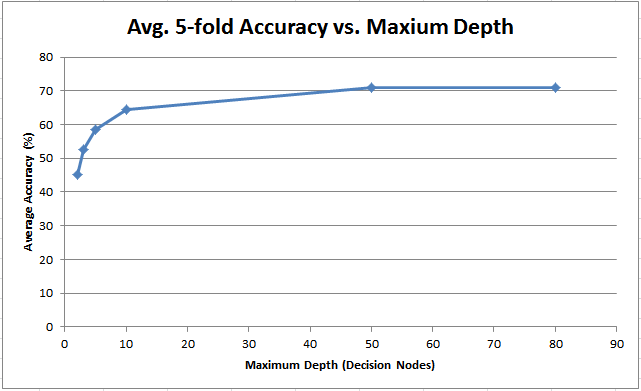
\includegraphics{3f.png}

The tree depth that results in the highest average accuracy is 50 decision nodes, which results in an average accuracy of 71.1\% for 5-fold cross-validation.
\end{enumerate}

\end{document}